\section{Scheduling}

\subsection{Rate Monotonic Scheduling (RM)}

Annahme:

\begin{itemize}
    \itemsep-.5em 
    \item All tasks that have hard deadlines are periodic.
    \item All tasks are independent.
    \item $d_i = p_i$ for all tasks.
    \item $c_i$ is constant and is known for all tasks.
    \item The time required for context switching is negligible.
\end{itemize}

\begin{minipage}[t]{.49\linewidth}
    \vspace{0pt}
    \formula{$\mu = \sum_{i=1}^{n}{\dfrac{c_i}{p_i}} \leq n ( \sqrt[n]{2} - 1 ) $}

    \unitText{$\mu$}{Auslastung}{1}\\
    \unitText{$n$}{Anzahl der Jobs}{1}\\
    \unitText{$c_i$}{Ausführungszeiten}{s}\\
    \unitText{$p_i$}{Periodenlängen}{s}
\end{minipage}\hfill
\begin{minipage}[t]{.25\linewidth}
    \vspace{0pt}
    \begin{tabular}{ c|c }
        $n$ & $\mu$ \\
        \hline
        1 & 1     \\
        2 & 0.828 \\  
        3 & 0.780 \\
        4 & 0.757 \\
       \end{tabular}
\end{minipage}\hfill
\begin{minipage}[t]{.25\linewidth}
    \vspace{0pt}
    \begin{tabular}{ c|c }
        $n$ & $\mu$ \\
        \hline
        5 & 0.743 \\
        6 & 0.734 \\
        7 & 0.728 \\
        8 & 0.724 \\
       \end{tabular}
\end{minipage}

Priorität: Kürzeste $c_i$, dann kürzeste $p_i$.


\subsection{Deadline Monotonic Scheduling (DM)}

\begin{minipage}[t]{.49\linewidth}
    \vspace{0pt}
    \formula{$\mu = \sum_{i=1}^{n}{\dfrac{c_i}{d_i}} \leq n ( \sqrt[n]{2} - 1 ) $}
\end{minipage}\hfill
\begin{minipage}[t]{.49\linewidth}
    \vspace{0pt}
    \unitText{$\mu$}{Auslastung}{1}\\
    \unitText{$n$}{Anzahl der Jobs}{1}\\
    \unitText{$c_i$}{Ausführungszeiten}{s}\\
    \unitText{$d_i$}{Deadline}{s}
\end{minipage}

Priorität: Kürzeste $c_i$, dann kürzeste $d_i$, dann kürzeste $p_i$.

\subsection{Earliest Deadline First (EDF)}

Es ordnet den Tasks Prioritäten zu, die sich nach der absoluten Deadline richten. Der Task, dessen Frist am nächsten ist, erhält die höchste Priorität.
Preemption möglich!

\begin{center}
    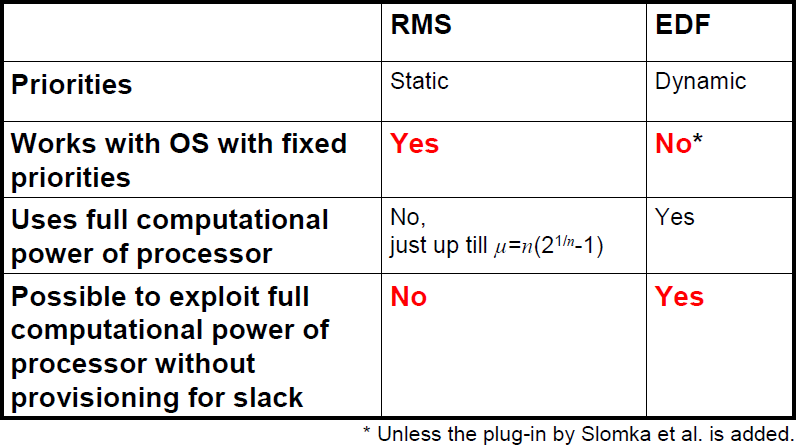
\includegraphics[width=.8\linewidth]{RMSvsEDF.png}
\end{center}


Oft werden Hybride verwendet:
\begin{center}
    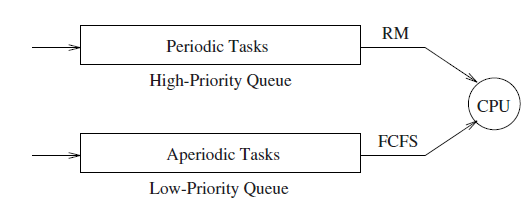
\includegraphics[width=.8\linewidth]{Scheduling_Hybrid.png}
\end{center}